\chapter[Chopin and Prelude, Op. 28, No. 15]{Frédéric Chopin - \textit{Prelude, Op. 28}, No. 15, the ``Raindrop'' Prelude (1838)}

Fryderyk Chopin (1810-1849) was a composer during the Romantic period (generally known to be from 1800-1910) who composed primarily for the piano. Born near Warsaw in a section of Poland which was at the time under Russian control, Chopin's clear talents as a musician were clear from an early age. By age seven, he had played his first public concert as a soloist, and had published his first piece. Over the course of years, his pieces would evolve to have a defined Polish character. In 1830, Chopin began touring through Germany and Italy, to gain an international reputation as a performer and composer, and settled in Paris, France in 1831. By this point, Chopin had already mostly reached fully compositional maturity. Four genres generally attributed to Chopin, the mazurka, étude, waltz, and polonaise, had matured by then, as Chopin had begun writing these in the 1820s\autocite{Burkholder_Grout_Palisca_2014}. The étude, a genre heavily associated with both Chopin and fellow Romantic-era composer Franz Liszt, is a piece which is intended to develop technique, or a certain skill on the instrument of choice, and only develops a singular figure through the piece. The other three genres that are known to be \say{Chopin genres} are stylized dances, typically for students, and are idiomatic in both figurations and fingerings\autocite{Burkholder_Grout_Palisca_2014}. Chopin's waltzes evoked the spirit of ballrooms in Vienna, but the mazurkas and polonaises are infused with Polish character. The polonaise is a type of courtly, and aristocratic dance, in $\frac{3}{4}$ time, also marked by a rhythmic figure of one eighth note and two sixteenth notes on beat one. The mazurka is a Polish folk dance, and in the time of Chopin, had become an urban type of ballroom dance, popular amongst those in high society in both Paris and Poland. Similar to the polonaise, the mazurka is in $\frac{3}{4}$ time, with accents on beats two or three, and a dotted figure of some kind on beat one. Mazurkas also feature a simple accompaniment, especially in the left-hand for piano, and combine four-bar long phrases into periods which alternate in A BA C form. The melody for a mazurka is also important, as it is instrumental in style, rather than vocal in style. This leads to elements of Polish instrumental folk music being prominent, and includes aspects solely found in melodies of instrumental music: large trills, grace notes, large leaps from one note to the next, and slurs to imitate the bowing found in traditional Polish folk songs. If articulated properly, a mazurka would sound uneven in tempo as it allows for ornamentations (such as the \textit{sforzando}, trills, and grace notes) to lengthen in time, and would lead to dancers to be able to execute turns or lifts. 

In the years before 1838, when the Raindrop Prelude was written, there was a brief, albeit interesting, period of Chopin's life. A period of writing, 1837 marked the year in which Chopin crossed paths with George Sand, a novelist later to be Chopin's partner, yet it was not until April 1838 in which they made this pairing official. The pair, along with Sand's children, spent the winter months of 1838-9 in Valldemossa, Majorca, an old Carthusian monastery. Recuperating from an illness and in the midst of a winter storm, Chopin began writing the 24-set preludes\autocite{Samson_2001}. Thus, the title of the fifteenth prelude of this set relates to the rain and stormy weather Chopin weathered while at Majorca, as well as the uncertainty regarding his health.

In 1838, Chopin wrote the set of 24 preludes, Opus 28, of which the fifteenth (simply known as the \say{Raindrop Prelude} is arguably one of the most famous of this set. Structurally, this prelude is in ternary form, with three sections: \textit{ABA}, and a coda. 

\begin{figure}[h]
  \centering
  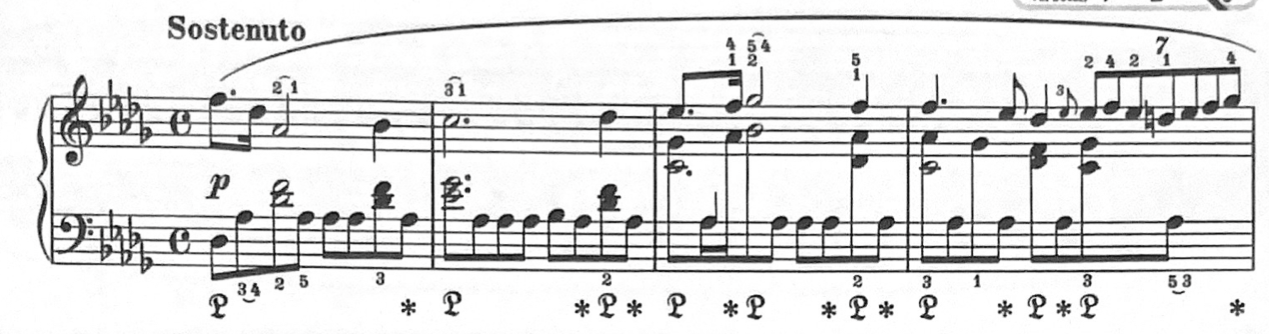
\includegraphics[width=\textwidth]{chopin-a-section-first-four-bars.jpg}
  \caption{The first four bars of Chopin's \textit{Prelude, Op. 28, No. 15}}
  \label{fig:chopin-a-section-first-four-bars}
\end{figure}

The first section, A, is a sweet section, reminiscent of gentle rain, akin to a sprinkle of rain. The delicate nature of this section is shown in the continuous usage of the \textit{piano} dynamic, as in Figure \ref{fig:chopin-a-section-first-four-bars}\autocite{Hansen_1973}. So, the performer playing this piece will play this section, as well as its related A' section, as the most expressive of the piece. As implied in bars three and four of Figure \ref{fig:chopin-a-section-first-four-bars}\autocite{Hansen_1973}, this typically becomes an interpretation in which there is a consistent usage of \textit{rubato}\autocite{Cole_Schwartzb}\footnote{A common practice in Romantic-era compositions. It involves taking a part of the duration of one note, and then giving it to another note. The performer is tasked with tastefully stretching, slowing, or hurrying the tempo, to their discretion. This gives the performer the greatest amount of flexibility and emotion available to interpret the piece.} and gradual crescendos and decrescendos to and from mezzo piano (medium loud). This is best seen when the piece in bars three and four ascend, peaking on the note G, and then descend, to a temporary low of D. This rise to G and subsequent fall to D will typically be played as a crescendo as the performer reaches the note G, and then a decrescendo back to \textit{piano} as the performer approaches the note D. The titular raindrop that this piece is named after is easily heard within the first three notes played in this piece and section: F, D\musFlat{}, and A\musFlat{}, outlining the piece's tonic key of D\musFlat{} Major. This phrase of three notes repeats again in other places in section A and A', as the raindrop motif, signifying the raindrops falling, and giving the section a melody which is cantabile and smooth. This section also features a repeated-note motif of the A\musFlat{} which is found in the left-hand, as in Figure \ref{fig:chopin-a-section-first-four-bars}\autocite{Hansen_1973} and many other places throughout A and A' sections. The raindrop motif stands out more against the background hum, or the sounds of other raindrops falling in tandem, which the left-hand's pedal point provides. The two motives here provide a texture which is entirely homophonic in this section. The texture solely consists of the right-hand melody, and the raindrop motif, and the left-hand's accompaniment, with the pedal point motive. This causes the section to sound thin in texture and timbre, as the right-hand provides its melody through the use of broken chords, and the left-hand provides a pedal note. Beyond the simplistic homophonic. texture, this section also contains tasteful ornamentations, featuring the use of rubato and other rhythmic ornamentation, among others, as shown by Figure \ref{fig:chopin-a-section-examples-ornamentation}\autocite{Hansen_1973}. At the end of the A section, there is a key change to the relative minor key of C\musSharp{} Minor, D\musFlat{} Major's relative minor key. This becomes the B section's tonic key.

\begin{figure}[h]
  \centering
  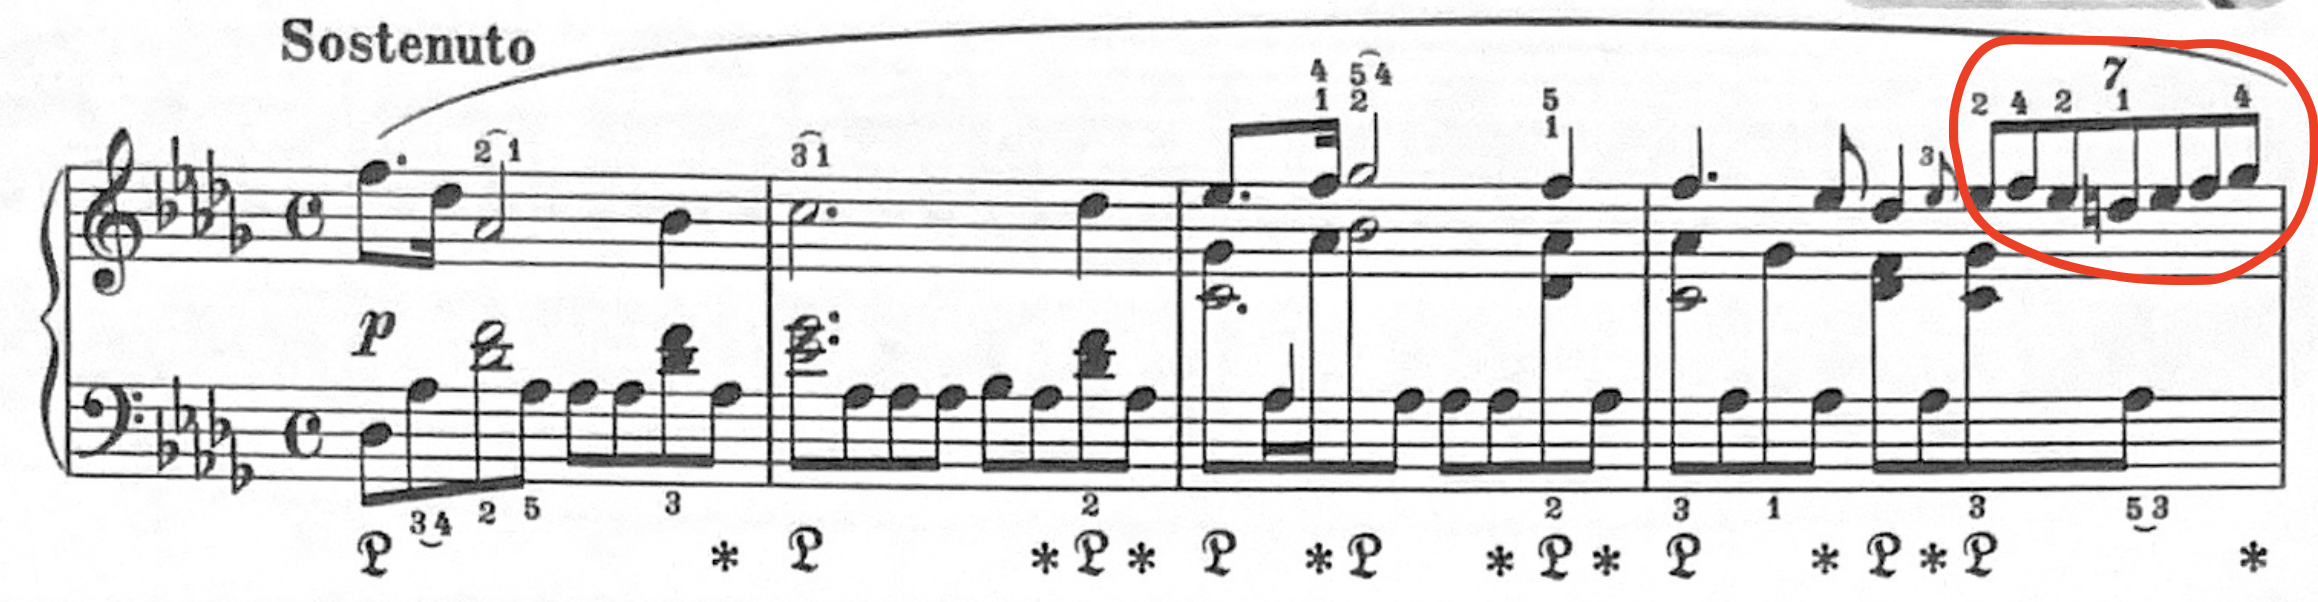
\includegraphics[width=\textwidth]{chopin-a-section-seven-note-run.jpg}
  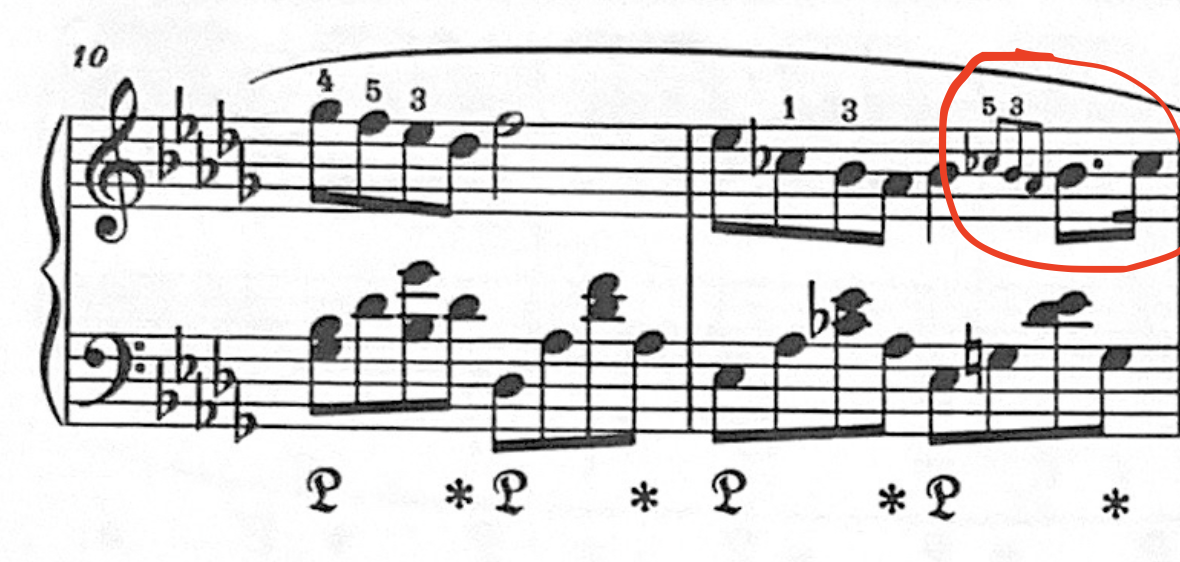
\includegraphics[width=\textwidth]{chopin-a-section-triplet-grace-note.jpg}
  \caption{Several examples of ornamentation, in Chopin's \textit{Prelude, Op. 28, No. 15}}
  \label{fig:chopin-a-section-examples-ornamentation}
\end{figure}

\begin{figure}
  \centering
  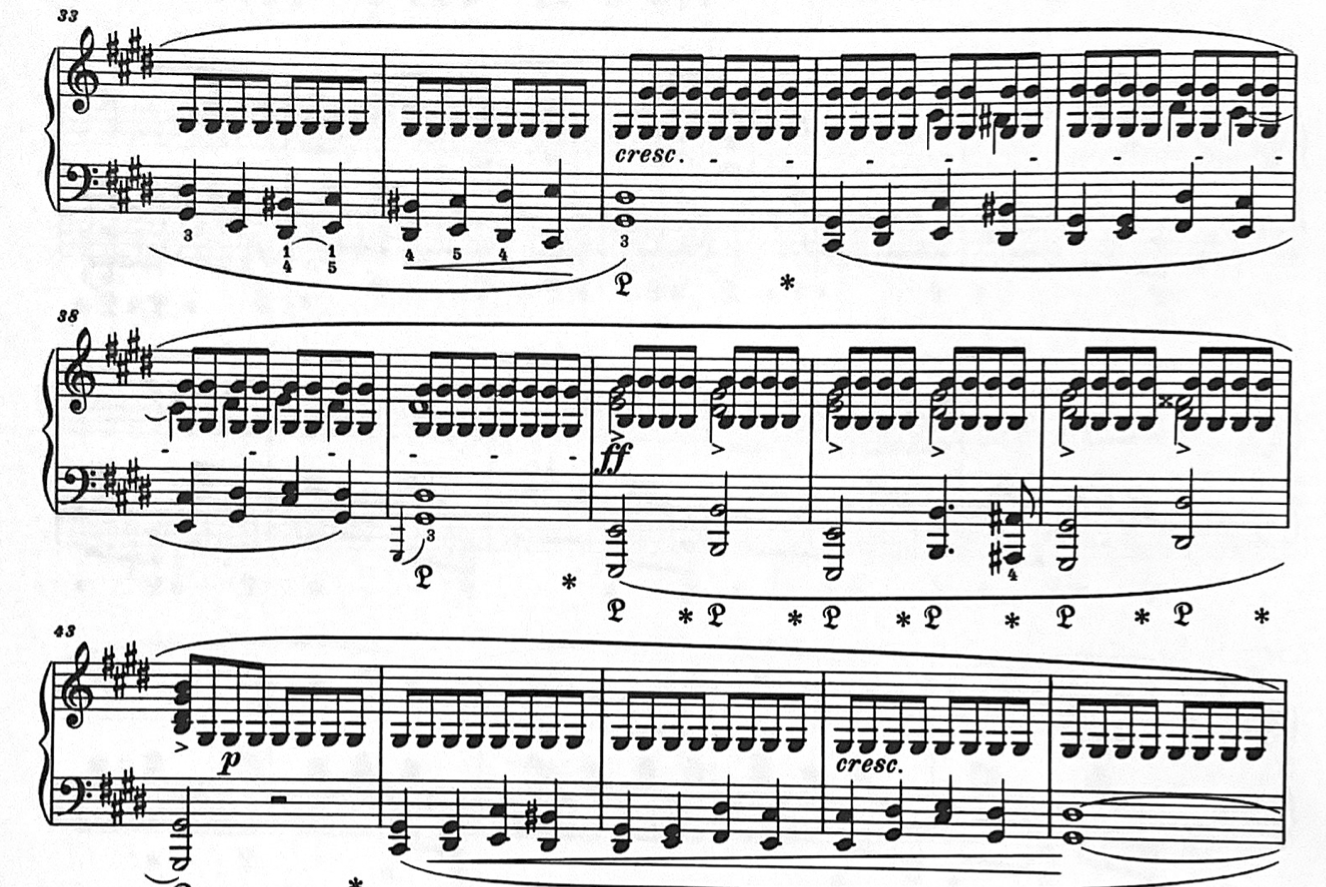
\includegraphics[width=\textwidth]{chopin-b-section-crescendos.jpg}
  \caption{The changes in dynamics, in Chopin's \textit{Prelude, Op. 28, No. 15}}
  \label{fig:chopin-b-section-crescendos}
\end{figure}

\begin{figure}
  \centering
  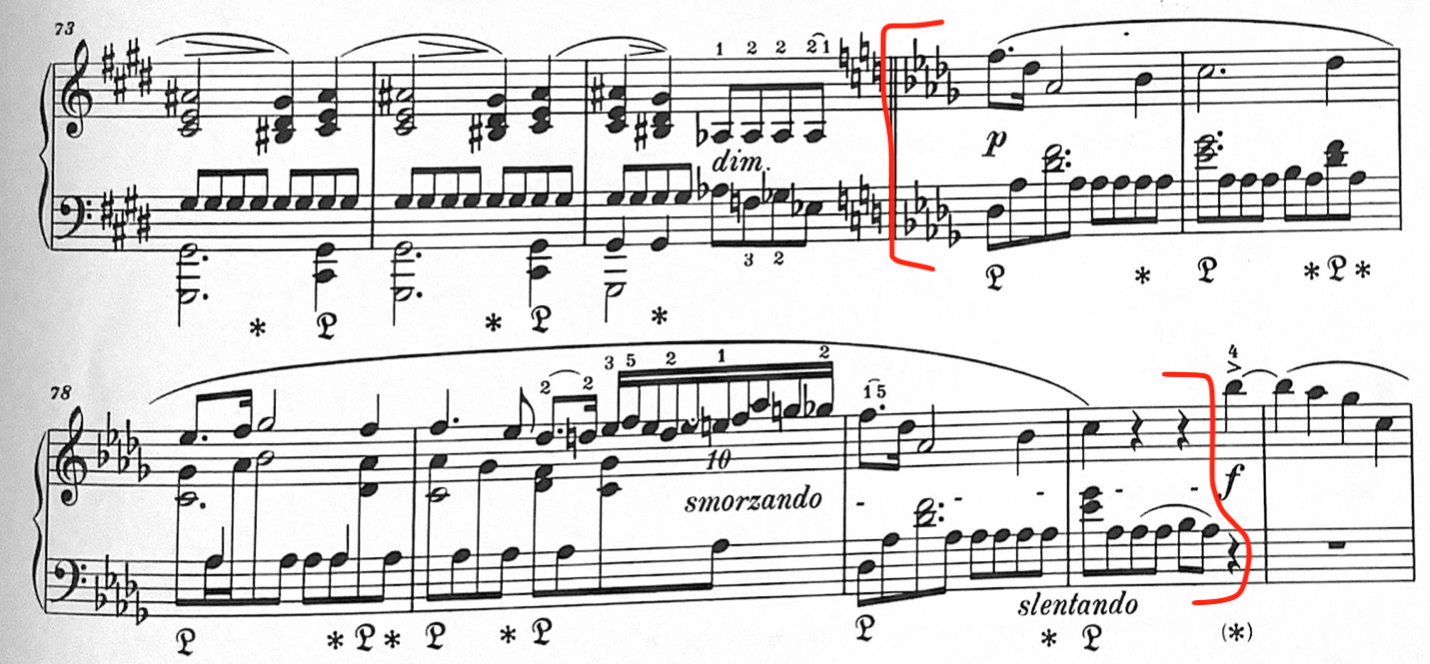
\includegraphics[width=\textwidth]{chopin-a-prime-section-ornamentation.jpg}
  \caption[Ornamentations in A', Chopin's \textit{Prelude, Op. 28, No. 15}]{The various ornamentations in the A' section of Chopin's \textit{Prelude, Op. 28, No. 15}}
  \label{fig:chopin-a-prime-section-ornamentation}
\end{figure}

\begin{figure}
  \centering
  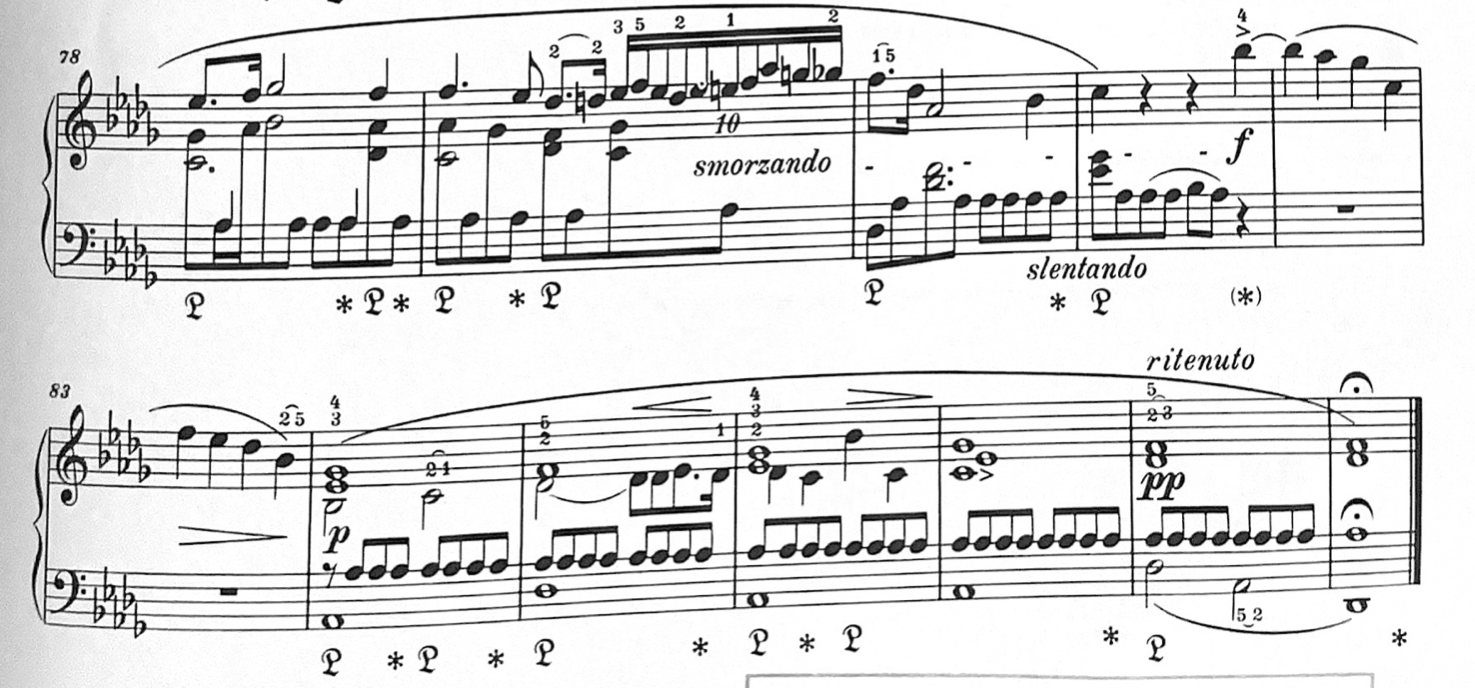
\includegraphics[width=\textwidth]{chopin-coda.jpg}
  \caption{The coda, Chopin's \textit{Prelude, Op. 28, No. 15}}
  \label{fig:chopin-coda}
\end{figure}



The B section is a high contrast to section A in character and tone. With the key change to C\musSharp{} Minor, the pedal note of A\musFlat{} turns into G\musSharp{}, and tension is introduced in this section. While section A's texture was a homophonic one, this section's texture is much more chordal, with chords featured in both hands, and also contains notes which are generally lower in pitch. Additionally, the repeated note motif is now in the right-hand, as it plays the note G\musSharp{}, in Figure \ref{fig:chopin-b-section-crescendos}\autocite{Hansen_1973}, creating a sort of ``inverted'' pedal point. The melody then shifts to the left-hand. As the section goes on, crescendos are used to build additional tension (see Figure \ref{fig:chopin-b-section-crescendos}\autocite{Hansen_1973} for reference, for example) as the dynamics increase from \textit{sotto voce} to \textit{fortissimo} ( \say{very loud}). The section begins \textit{sotto voce} (``under the voice'', which has similar meaning to \textit{piano}), and gradually builds with crescendos\footnote{Figure \ref{fig:chopin-b-section-crescendos}}\autocite{Hansen_1973}. As the tension builds, the left-hand also adds slurs as ornamentation, adding a legato effect to the notes which also contributes to the rising tension. Once the dynamics peak at \textit{fortissimo}, the volume drops to \textit{piano} and repeats the section again. Dynamics are the primary tool used by the performer to add their interpretation and expression to the piece in this section, and the \textit{fortissimo} is used to great effect when the crescendo builds, and is at its highest when we arrive at the chords of E Major and B Major.

The return of the A section, although a modified version, returns the original melody of the first A section. It return \textit{piano}, and is also marked \textit{smorzando} (``dying away'') to signify the intended ending in \textit{pianissimo} (very soft). The first A section's tonic key of D\musFlat{} Major returns, and so does a majority of the ornamentation decisions, including rubato, and other decorations which are explored more deeply, as in Figure \ref{fig:chopin-a-prime-section-ornamentation}\autocite{Hansen_1973}. However, we only hear the first eight bars of this second A section, as Chopin includes a coda to finish the piece.

This coda (or more accurately, codetta, a short coda) finishes the prelude. As seen in Figure \ref{fig:chopin-coda}\autocite{Hansen_1973} and marked in red brackets, there are elongated quarter notes which descend, played in \textit{forte} (loud), to add a sense of both intensity and delicacy to the ending. In the third full bar of the coda, the pedal point is reintroduced, this time as A\musFlat{}, played in the right-hand. It, like its role in the first A section, is like that of falling raindrops, serving as a background sprinkle for this ending. The coda ending is marked with the word \textit{ritenuto}\autocite{Cole_Schwartza}, to indicate the sudden slowing of the tempo, almost an extreme slowing of the tempo. With the \textit{ritenuto}, it is a clear ending to this prelude, and is akin to the ending of a rainstorm, in which the rain clears up.

\section{...But He's Supposed to be Dead!}\label{section:chopin-interpretation}

Chopin wrote this prelude during one particularly brutal winter, in Valldemossa, Majorca. This prelude is number fifteen of the twenty-four set of preludes. As its title ``Raindrop'' suggests, the fifteenth prelude relates to the rain and stormy weather which Chopin was subject to during his time alone in Majorca. There was uncertainty regarding his health, and this is clearly seen in all aspects of the piece.

In the very first measure of the piece, in the A section, we note two things. First, that Chopin has set the dynamic marking of the piece's beginning to be \textit{piano}, with the right-hand melody meant to be played smoothly. Second, that the first three notes played in the right-hand, as in Figure \ref{fig:chopin-a-section-first-four-bars}\autocite{Hansen_1973}, emulates the sound of raindrops falling. There is the rhythm of a dotted eighth note, followed by a sixteenth note and a half note. This places the sound of the falling rain at the center of the piece, as a melodic motif that a listener can easily decipher. Thus, I play it out, fading the left-hand harmony into the background, as this is the central motif to the entire prelude. The left-hand harmony becomes the low murmur of rain hitting the roof of a home, and the soprano notes (the highest notes which sound in the right-hand) become more pronounced, as the melody rises and falls. Other dynamic markings which Chopin includes in the A section of this piece are also instrumental to my performance of this section as warm and lulling in nature. As the melody line in the right-hand rises and falls, I match each peak and dip in melody with its appropriate dynamic contrast; when the melody rises and peaks at the note G (as it does in Figure \ref{fig:chopin-a-section-first-four-bars}\autocite{Hansen_1973}), I increase the dynamic of the melody to its loudest, and do the same with the lowest note D, decreasing my dynamic to its lowest. Additionally, as mentioned, while I choose not to place emphasis on any of the notes below Middle C, I play the left-hand as warm and as full as I can, to encapsulate the nature of a violent wind and rainstorm happening outside, the way Chopin might have heard it. It is easy to play the melody out against a soothing backdrop of rain patter, as it acts as a pedal point through which the listener can focus on other sounds instead.

Beyond the literal representation of the windstorm happening to Chopin while at the Carthusian monastery he stayed at in 1838-9, the A (and later, A') section is also meant to represent Chopin's fear of death and dying alone without his loved ones near. As in Figure \ref{fig:chopin-a-section-examples-ornamentation}\autocite{Hansen_1973}, in addition to the raindrop motif frequently reoccurring in various iterations, there is also the use of other ornamental tools which I use to highlight Chopin's unease with facing his mortality. There is a clear fear of death, which I present through placing greater emphasis and rubato on three-note phrases which include a dotted eighth note and sixteenth note. In addition, there are also several passages, such as in measure 11 of Figure \ref{fig:chopin-a-section-examples-ornamentation}\autocite{Hansen_1973}, in which triplets, and three- to seven-note grace notes, allude to the uncertainties regarding death. Within phrases which contain either three-note grace notes or seven-note grace notes, I play these quicker, with a slight bounce to them. This again emphasizes the intense fear of death Chopin had, as well as the unknown regarding aspects of medicine and sickness in the seventeenth century.

As the A section transitions into the B section, there is a change in texture, timbre, and overall sound quality. I follow this transition in sound, placing greater emphasis on the left-hand's bass notes, and bringing the dynamic level of the left-hand harmony to equal that of the right-hand. When the B section begins, as in Figure \ref{fig:chopin-b-section-crescendos}\autocite{Hansen_1973}, the dynamic volume is still piano, and the right-hand plays either single notes, octaves, or a combination of both. I maintain the same steady increase and decrease in dynamic volume as I did in the A section, as I begin the B section playing \textit{piano}, and slowly yet dramatically increase the volume as the crescendos note. Chopin had far more anxieties about his health, which comes across in this section. The first two measures of the B section start off tame in comparison to the latter half of the section, as the right-hand creates a pedal point on the note G\musSharp{}, while the left-hand plays a \textit{dyad}, or a two-note chord. These anxieties slowly fester within Chopin, and become ``louder'' in volume, as does the section's dynamics, with the five-measure long crescendo, peaking at a rambunctious and resounding \textit{fortissimo}. Within the music, there is little action, but I sound it to appear at least twice as complex. With the left-hand slowing in its action (from dyad quarter notes to the octave half notes, with occasional dotted quarter notes and eighth notes), the right-hand melody gains movement. Between measures 36-38, on beats three and four in Figure \ref{fig:chopin-b-section-crescendos}\autocite{Hansen_1973}, the right-hand octaves also feature two slurred quarter notes. These change to become dyad half notes, which sound under the right-hand's octaves. 

It is here, in measures 40-42, where the emotional climax of the piece lies. On beat one of bar 40, the left-hand plays a loud and dramatic half note, holding on the note E, while the right-hand plays four eighth note octaves on B, while also holding a half note dyad on E and G\musSharp{}. It is heavy, and intense, and provides a sharp contrast to the material treated in both the A  section, and the first seven bars of the B section. The rain is coming down much harder, and the wind is howling, which I emulate through the half notes that sound in the right-hand. These half notes are noticeable, but do not draw the listener's attention away from the octaves the right-hand plays. Once the left-hand introduces its octaves to be played in bar 34 in Figure \ref{fig:chopin-b-section-crescendos}\autocite{Hansen_1973}, there is a certain dramatization of the acceptance of death Chopin goes through. In the dynamic level of \textit{fortissimo}, there are accents on beats one and three (Figure \ref{fig:chopin-b-section-crescendos}\autocite{Hansen_1973}) and the half notes in the left-hand are complemented by the right-hand's half notes, creating a sound akin to the resounding Castillo gong in the Carthusian monastery. As the half notes are being held to their full duration, and I play the right-hand's octaves on top of the half notes, I emphasize the nature of the half notes, similar to the gong sounding in a monastery. The phrase in measures 40-42 portray Chopin's fear about death, as the gong sounding gets louder and also somehow closer to the listener, as it comes closer to him. This gong sound comes back later in the section, and alternates in thematic material treated, between the build-up of the rain and the wind, the dynamic marking returns to be \textit{piano}, and the left-hand resuming its prior movement. 

When the A section returns (in the form A'), bracketed in red in Figure \ref{fig:chopin-a-prime-section-ornamentation}\autocite{Hansen_1973}, the treated melodic material is mostly the same, except for ornamental changes. The rain and wind have decreased in intensity, and the difference between the end of the B section and the beginning of the A' section is stark. While the last few measures of the B section (bars 73-75 in Figure \ref{fig:chopin-a-prime-section-ornamentation}\autocite{Hansen_1973}) were dramatic, rambunctious, and referred to Chopin's uncertainty and fear about his own mortality, the beginning of the A' section is the calm reprieve for both the listener and Chopin. The first major change between the A' and the A section is the ten-note long sixteenth note phrase in bar 79 of  \ref{fig:chopin-a-prime-section-ornamentation}\autocite{Hansen_1973}, indicating the rain has not fully finished falling yet, nor has Chopin accepted the possibility of his death. 

The coda of the A' section, in Figure \ref{fig:chopin-coda}]\autocite{Hansen_1973}, is when I emphasize the finality that Chopin has, accepting the calm after the storm, as well as the possibility of his death. In beat four of bar 81 through the bracketed passage in red of Figure  \ref{fig:chopin-coda}]\autocite{Hansen_1973}, the left-hand harmony disappears, as the right-hand sounds alone for the first two measures. Played \textit{forte}, I interpret this to not only literally be the calm after the storm, but also a figurative rainbow which appears after the rain has stopped, and the sky has cleared. The only sounds for the first two full measures of the coda contain quarter notes, slurred into one another, and played \textit{forte}. It is the sudden appearance of a rainbow, like those that happen in the media, and which brightens the sky and clears Chopin, and the listener, of fears regarding death. Instead, both Chopin and the listener are transported into an acceptance of the inevitable, and are able to see the beauty in the calm. This acceptance is not overdramatized by my performance, as I keep the dynamic level of bar 84 to the end at a \textit{piano}, and let the melody and harmony lines perfectly balance each other. The whole notes in the left hand ground the right-hand's melody, while the eighth notes in the left-hand emphasize the acceptance of death and the beauty of the rainbow, and do not overstate its importance. The addition of the pedal, starting in bars 84 (Figure \ref{fig:chopin-coda}\autocite{Hansen_1973}) also adds to the air of acceptance and inner peace, as the coda ends with the word \textit{ritenuto}. The extreme slowing of tempo and shift to a dynamic of \textit{pianissimo} symbolizes this recognition and compliance, as it ends with satisfied whole note dyads in both hands, and a fermata elongating the notes' durations.
%
%Could also tie in idea of rain and the literal rain interpretation with the intense fear of death \& eventual acceptance with the calm after a heavy rain \& stereotypical rainbow afterwards